\documentclass[12pt, fullpage,letterpaper]{article}

\usepackage[margin=1in]{geometry}
\usepackage{url}
\usepackage{amsmath}
\usepackage{tikz}
\usetikzlibrary{fit,calc,arrows,positioning}
\usepackage{stackengine}
\usepackage{caption}
\usepackage{subcaption}
\usepackage{graphicx}
\usepackage{algorithmic}
\usepackage{algorithm}
\usepackage{pdflscape}
\usepackage{longtable}

\newcommand{\semester}{Fall 2015}
\newcommand{\assignmentId}{4}
\newcommand{\releaseDate}{Nov 3, 2015}
\newcommand{\dueDate}{Nov 17, 2015}

\newcommand{\bx}{{\bf x}}
\newcommand{\bz}{{\bf z}}
\newcommand{\bw}{{\bf w}}

\title{CS 5350/6350: Machine Learining \semester}
\author{Homework \assignmentId\\ Christopher Mertin}
\date{Handed out: \releaseDate\\
  Due date: \dueDate}

\begin{document}
\maketitle

\section*{General Instructions}

{\footnotesize
  \begin{itemize}
  \item You are welcome to talk to other members of the class about
    the homework. I am more concerned that you understand the
    underlying concepts. However, you should write down your own
    solution. Please keep the class collaboration policy in mind.

  \item Feel free ask questions about the homework with the instructor
    or the TAs.

  \item Your written solutions should be brief and clear. You need to
    show your work, not just the final answer, but you do \emph{not}
    need to write it in gory detail. Your assignment should be {\bf no
      more than 10 pages}. Every extra page will cost a point.

  \item Handwritten solutions will not be accepted.

  \item The homework is due by midnight of the due date. Please submit
    the homework on Canvas.

  \item Some questions are marked {\bf For 6350 students}. Students
    who are registered for CS 6350 should do these questions. Of
    course, if you are registered for CS 5350, you are welcome to do
    the question too, but you will not get any credit for it.

  \end{itemize}
}

%%% Local Variables:
%%% mode: latex
%%% TeX-master: "hw2"
%%% End:
\section{Warm up: Support Vector Machines}
\label{sec:svm}

In class you have seen support vector machines (SVMs).  Here we will find the optimal classifier of a simple dataset by hand.  Assume that we are given the following dataset:
\begin{align*}
\mathcal{D}_+ &= \begin{bmatrix}
  3 & \phantom{-}1\\
  3 & -1\\
  6 & \phantom{-}1\\
  6 & -1
\end{bmatrix}
&& \mathcal{D}_-= \begin{bmatrix}
  \phantom{-}1 & \phantom{-}0\\
  \phantom{-}0 & \phantom{-}1\\
  \phantom{-}0 & -1\\
  -1 & \phantom{-}0
\end{bmatrix}
\end{align*}
where $\mathcal{D}_+$ are positive examples and $\mathcal{D}_-$ are negative examples.
\begin{enumerate}
\item ~[9 points] Find the optimal hyperplane and the corresponding
  maximum margin. Which training points are the support vectors?

\begin{itemize}
\item The solution is the hyperplane about $y=2$, which can be seen in Figure~\ref{fig:1a}, where the support vectors are from the positive as $(3,1)$ and $(3,-1)$ as they both have the same distance to the hyperplane, and for the negatives $(1, 0)$. It is the maximized margin between both points (the midpoint between them) as the distance of each closest point to the hyperplane is $1$.
\end{itemize}

\item ~[2 points] You are given a new point $x = [1.8,1]$ with true
  label -1. Does your SVM correctly classify this point?

\begin{itemize}
\item Yes, please refer to Figure~\ref{fig:1b}
\end{itemize}  



\item ~[4 points] Now let's compare this classifier to the vanilla
  Perceptron algorithm. Assume that we have the point $x = [1.9999,1]$
  with label -1. If we allow the Perceptron algorithm to run until it
  achieves 0\% error on the training set will it be guarenteed to
  classify this point correctly? Why or why not justify your answer.

\begin{itemize}
\item I talked with Dr. Srikumar and he said that this question is to be taken as you {\em learn} on the original 8 points, and the $(1.999,1)$ point is to be the ``test'' point. 

The vanilla Perceptron algorithm will not necessairly classify the last point correctly. The normal Perceptron algorithm does not care about the resulting weight vector, only that the training set is classified correctly. Figure~\ref{fig:1c} shows and example of how the training set could be classified correctly, but it wouldn't classify the test point $(1.999,1)$ correctly.
\end{itemize}  


\end{enumerate}

\begin{figure}[!h]
\centering
\begin{minipage}{.5\textwidth}
  \centering
  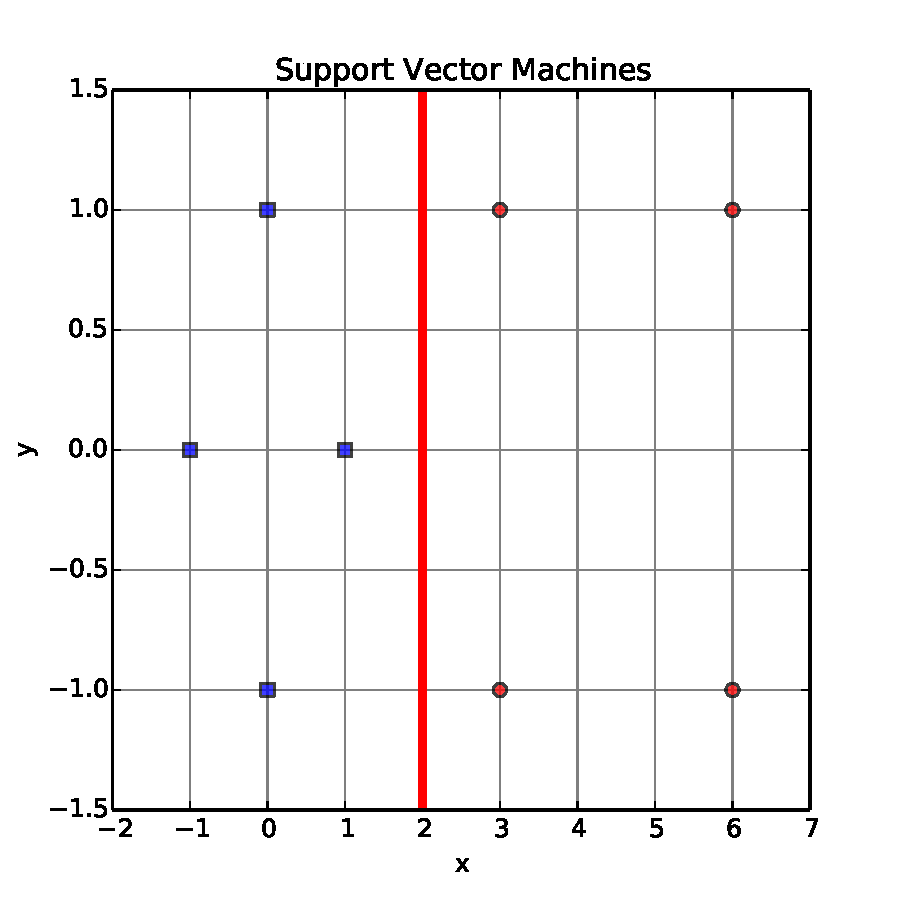
\includegraphics[width=\linewidth]{progs/1a.pdf}
  \captionof{figure}{Solution to Problem 1}
  \label{fig:1a}
\end{minipage}%
\begin{minipage}{.5\textwidth}
  \centering
  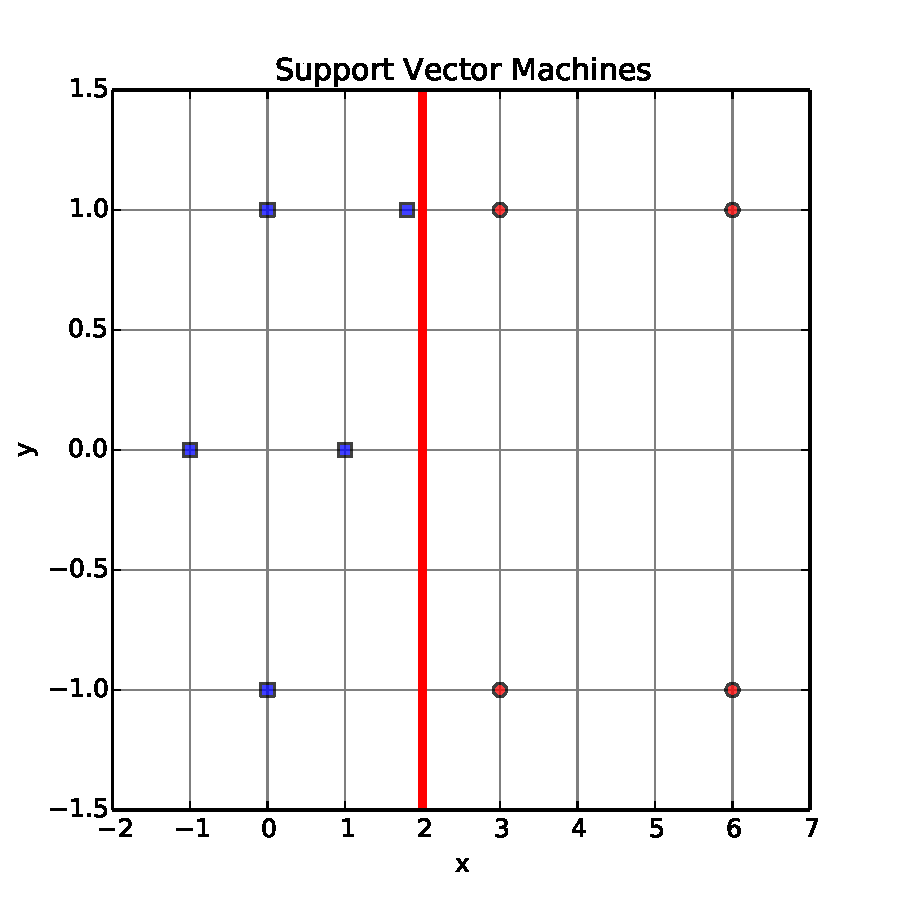
\includegraphics[width=\linewidth]{progs/1b.pdf}
  \captionof{figure}{Solution to Problem 2}
  \label{fig:1b}
\end{minipage}
\end{figure}

\begin{figure}[!h]
\centering
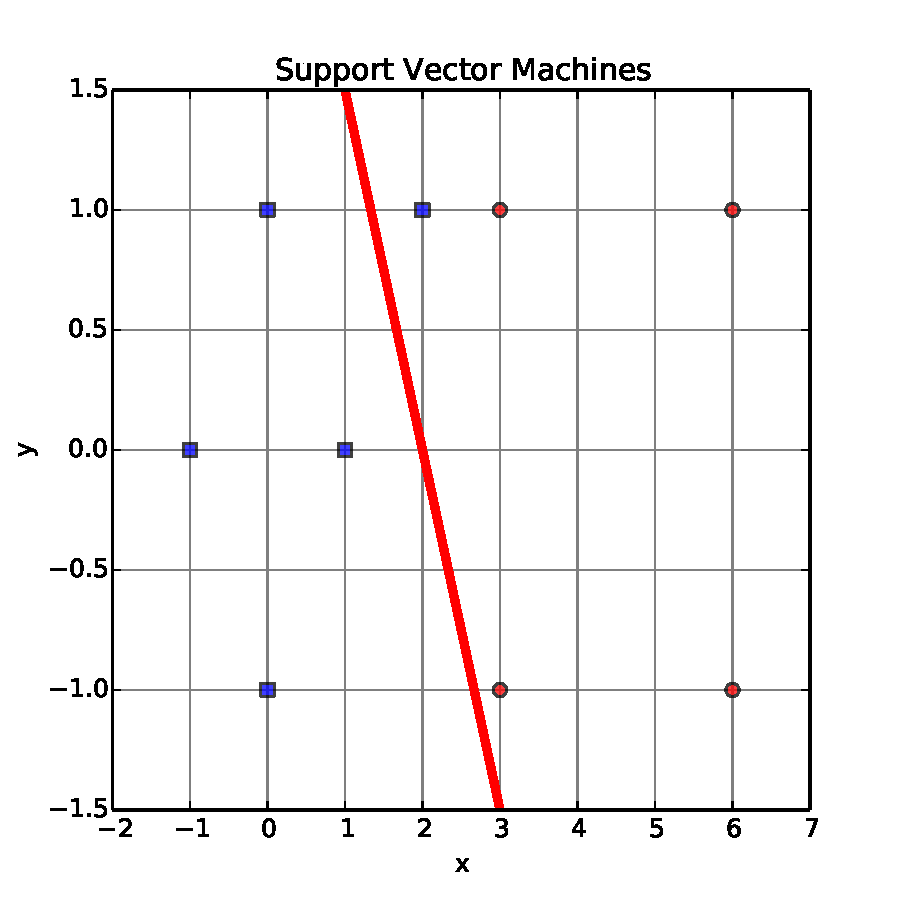
\includegraphics[width=.5\linewidth]{progs/1c.pdf}
\caption{Solution to Problem 3}
\label{fig:1c}
\end{figure}


%%% Local Variables:
%%% mode: latex
%%% TeX-master: "hw4"
%%% End:

\section{Kernels and the Perceptron algorithm}
\label{sec:kernel}

In the class, we saw how the idea of kernels can be applied to
increase the expressiveness of the SVM classifier. Kernels is more
broadly applicable than just SVMs. In this question, we will see how
kernels can be used with the Perceptron algorithm.

Suppose, we wish to learn a $k$-DNF (not necessarily monotone) using a
kernel version of Perceptron. Recall that a $k$-DNF is a Boolean
function that is a disjunction of conjunctive clauses, where each
conjunctive clause has exactly $k$ literals. For example, the
following Boolean functions are $2$-DNFs:
\begin{itemize}
\item $(x_1 \wedge x_2) \vee (\neg x_2 \wedge x_3)$
\item $(\neg x_1 \wedge x_2) \vee (x_3 \wedge x_4) \vee (\neg x_4 \wedge x_1)$
\end{itemize}

In order to learn a $k$-DNF, we will define a feature transformation
$\phi(\bx)$ that maps examples $\bx \in \{0,1\}^n$ to a new space of
$k$-conjunctions and then define a kernel Perceptron algorithm for
learning. That is, each element of $\phi(\bx)$ corresponds to the
value of a different $k$-conjunction and $\phi$ enumerates over all
$k$-conjunctions. After this transformation, the classification of the
Perceptron is via the sign of the dot product of the weight vector and
the example $\bw^T\phi(x)$. The goal is to represent this dot product
using a kernel $K(w, x)$.


\begin{enumerate}
\item ~[5 points] Show that any $k$-DNF is linearly separable after
  the feature transformation.

\begin{itemize}
\item As was proven in the last homework, $k$-Decision Lists ($k$-DL) are linearly separable. Therefore, this can be proven by showing that $k$-DNF functions are similar to that of $k$-DL's.

Assume we can have an arbitrary $k$-DNF of the form $f = \vee_{i=1}^{N}c_{i}$, where $c_{i}$ is a $k$-conjunction. We can turn this into a $k$-DL by the following form $C = \left\{(c_{1},1),(c_{2},1),\ldots,(c_{N},1),0  \right\}$. From this definition, it is easy to see that {\em both} $C$ and $f$ are satisfied as long as one of the $k$-conjunctions are true. Therefore, the $k$-DL and $k$-DNF behave in the same way, so the new $k$-DL can be used to make it linearly separable.
\end{itemize} 

\item ~[10 points] Let $C$ be the set of all conjunctions containing
  exactly $k$ different literals. (Recall that a literal is a Boolean
  variable or its negation.) For any $\bx_1, \bx_2 \in \{0, 1\}^n$,
  define
  $$K(\bx_1, \bx_2) = \phi(\bx_1)^T\phi(\bx_2) = \sum_{c \in C} c(\bx_1)c(\bx_2).$$ 

  Here $c(\bx)$ is the value of a conjunction $c$ using the values in
  $\bx$. Show that this function can be computed efficiently without
  explicitly computing the values of $\phi(\bx_1)$ and $\phi(\bx_2)$.

\begin{itemize}
\item The function can be efficiently computed in {\em linear time} as follows.

There are $\mathcal{O}(N)$ $k$-conjunctions $\in\ C$, which would be the upper bound on simply calcualting each of the conjunctions istead of worrying about mapping to the new space and taking the dot product. Since they are conjunctions, $c\left(\mathbf{x}_{1}\right)c\left(\mathbf{x}_{2}\right)=1$ when $c\left(\mathbf{x}_{1}\right)$ {\em and} $c\left(\mathbf{x}_{2}\right)$ are {\em both} true. Therefore, instead of mapping all of the data to the new feature space and taking the dot product, {\em at most} linear time can be achieved by simply looking at the ones with the same number of active features between the two sets and summing over those which agree.
\end{itemize} 

\item ~[5 points] Assume that the initial weight vector for Perceptron
  is the zero vector. Then, show that
  $\bw = \sum_{(\bx_i, y_i) \in M} y_i \, \phi(x_i)$. Here
  $M = \{(\bx_i, y_i)\}$ is the set of examples on which the learning
  algorithm made mistakes.

\begin{itemize}
\item The Perceptron algorithm only updates everytime it makes a mistake. To update the weight vector, it updates it as $\mathbf{w}_{i+1} = \mathbf{w}_{i} + y_{i}\mathbf{x}_{i}$. If we have a function $\phi(\mathbf{x})$ that maps $\mathbf{x}$ to a new feature space, we have $\mathbf{w}_{i+1} = \mathbf{w}_{i} + y_{i}\phi(\mathbf{x}_{i})$. If the Perceptron algorithm makes $M$ errors, the resulting weight vector can be reprsented as $\mathbf{w} = \sum_{(\mathbf{x}_{i},y_{i})\in M} y_{i}\phi(\mathbf{x}_{i})$.
\end{itemize} 

\item ~[5 points] Using the fact that the weight vector can be written
  as in the previous question, write the classification step
  $y=sgn\left(\bw^T\phi(\bx)\right)$ using the kernel function
  $\kappa(\bx_1,\bx_2)$ instead of using the explicit feature
  representations.

\begin{itemize}
\item From the question we have

\begin{align*}
y &= sgn\left( \mathbf{w}^{T}\phi\left(\mathbf{x} \right)\right)\\
\intertext{Which can be generalized by plugging in for $\mathbf{w}$ from the question before as}
y &= sgn\left( \sum_{(\bx_i, y_i) \in M} y_i \, \phi(\mathbf{x}_i)^{T}\phi(\mathbf{x})\right)\\
\intertext{We also know from the notes that $\kappa(\mathbf{x},\mathbf{z}) \equiv \phi(\mathbf{x})^{T}\phi(\mathbf{z})$. So we can use this to rewrite it in the form}
y &= sgn\left(\sum_{(\bx_i, y_i) \in M} y_i \, \kappa(\mathbf{x}_{i},\mathbf{x}) \right)
\end{align*}
\end{itemize} 

\item ~[15 points] Write explicitly the pseudo code for the kernel
  Perceptron algorithm that uses your kernel to learn a $k$-DNF.
  (Hint: Instead of storing the weight vector, you will store a list
  of examples where the algorithm makes mistakes.)

\begin{itemize}
\item The given problem states that the initial weight vector is the zero vector, therefore there is no bias term to account for in the update, so it will be ignored.

\begin{algorithm}
\caption{Zero'd Kernel Perceptron}
\begin{algorithmic}
\STATE $\mathbf{w}\leftarrow 0$
\FOR{$i=1$ \TO $M$}
    \IF{$y\neq sgn\left( \sum_{\bx_{i},y_{i}\in M} y_{i}\kappa(\mathbf{x},\mathbf{x}_{i})\right)$}
       \STATE{$\mathbf{w}\leftarrow \mathbf{w}\cup(\mathbf{x}_{i},y)$}
    \ENDIF
\ENDFOR
\RETURN $sgn\left( \sum_{\bx_{i},y_{i}\in M} y_{i}\kappa(\mathbf{x},\mathbf{x}_{i})\right)$
\end{algorithmic}
\end{algorithm}
\end{itemize} 
\end{enumerate}


%%% Local Variables:
%%% mode: latex
%%% TeX-master: "hw4"
%%% End:

\subsection*{Experiments}

For all your experiments, you may choose whatever hyper-parameters you
like, but we suggest that you informally experiment with them before
submitting the results. (You can use cross-validation to find the
hyper-parameters as you did in the previous homework. Note that we did
not partition the data into parts, so you should do that if you want
to find hyper-parameters using cross-validation.)

\begin{enumerate}

\item ~[Sanity check, 5 points] Run the simple Perceptron algorithm on
  the data in Table 2 (one pass only, without shuffling) and report
  the weight vector that the algorithm returns. How many mistakes does
  it make?

  \verb~Sanity Check. Running Perceptron Algorithm on Table 2~

  \verb~Number of Updates: 4~

  \verb~Weight Vector: [ 0.   0.1  0.1  0.1]~

  The given weight vector accuracy classifies the data. It does require
  $x_2,\ x_{3},\ x_{4}$ to be greater than 0 to be classified when the actual
  function only requires $x_{4}$ to be positive. Thus it included extra
  ``features'' to the data which don't really effect the final result since
  the classification is only dependent upon the value of $x_{4}$.


\item ~[Online Perceptron, 15 points] Choose the 10 dimensional
  training set ({\tt train0.10}) from the {\tt data0} folder and its
  corresponding test dataset. Run both the Perceptron algorithm and
  the margin Perceptron on this dataset for one pass. Report the
  number of updates (or equivalently mistakes) made by each algorithm
  and the accuracy of the final weight vector on both the training and
  the test set. Once again, you will require some playing with the
  algorithm hyper-parameters. You will see that the hyper-parameters
  will make a difference and so try out different values.

  \verb~Running over the 10-Dimensional data~

  \verb~Normal Perceptron~

  \verb~Updates: 35 Accuracy: 1.0~

  \verb~Margin Perceptron~

  \verb~Updates: 33 Accuracy: 1.0~

  For this instance, the Perceptron and the Margin Perceptron algorithm were
  used on the 10 dimensional data set in the \verb~d0~ file. For each of these
  functions, there was an initial weight vector $w$ that was randomly generated
  to use as the initial starting point of the weight vector for each algorithm.

  For the Normal
  Perceptron Algorithm, what was done was a list of the learning rate $r$
  was given in the range from $[0.1,1]$. Each value was tested with the
  Perceptron Algorithm, and the value for $r$ that gave the least number
  of updates was returned. The least number of updats was choosen because
  this implies that the weight vector that was created would also not need
  as many updates when classifying future data (test data) if it's relatively
  the same. As can be seen in the above output, the Normal Perceptron Algorithm
  needed \verb~35~ updates and was able to correctly classify all of the data
  in the test file.

  When doing the Margin Perceptron Algorithm, a list of learning rates for $r$
  and $\mu$ was choosen, where $r$ was in the range $[0.1,1]$ and $\mu$ was
  constrained to $[0, 0.1]$. The ranges for both of these were determind by
  multiple trials and seeing which one classified better. The same technique
  was used for choosing the hyper-parameters, except in this instance each
  combination of $r$ and $\mu$ were looked at. After determining the
  hyper-parameters, the Margin Perceptron algorithm was run with them and the
  weight vector to classify the data was returned. As can be seen above, the
  Margin Perceptron Algorithm did it in slightly less number of updates,
  \verb~33~ when compared to \verb~35~, and also successfully classified all
  of the test cases.


\item ~[Batch Perceptron on all datasets, 40 points] Now, on each
  train/test dataset in the {\tt data0} and {\tt data1} folders, run
  the Perceptron and margin Perceptron algorithms for ten epochs. {\em
    Do not forget to randomly shuffle the data at the start of each
    epoch.}

  Record the the number of updates on the train datasets and the
  accuracy on the test data sets.

  So, for example, use the {\tt data0/train0.10} file to train your
  Perceptron and test it on {\tt data0/test0.10} and record the number
  of updates/mistakes and accuracy. Then, repeat this for all other
  datasets. This constitutes one experiment. Once you have the above
  data, plot two sets of graphs for each experiment ({\tt data0}/{\tt
    data1} + Perceptron/margin Perceptron):
  \begin{center}
    \begin{tikzpicture}[scale=0.6]
      % Axis
      \draw[->,>=latex'] (0,0) -- coordinate (x axis mid) (6.5,0);
      \draw[->,>=latex'] (0,0) -- coordinate (y axis mid) (0,6.5);
      % Labels
      \node[below=0.2] at (x axis mid) {dimension};
      \node[rotate=90,yshift=10pt] at (y axis mid) {number of
        updates}; % Or use above alone.

    \end{tikzpicture}
  %
    \begin{tikzpicture}[scale=0.6]
      % Axis
      \draw[->,>=latex'] (0,0) -- coordinate (x axis mid) (6.5,0);
      \draw[->,>=latex'] (0,0) -- coordinate (y axis mid) (0,6.5);
      % Labels
      \node[below=0.2] at (x axis mid) {dimension};
      \node[rotate=90,yshift=10pt] at (y axis mid) {test set
        accuracy}; % Or use above alone.

    \end{tikzpicture}
  \end{center}

  For the results of this part, please look at question 4 as I decided to
  include the Agressive Margin Perceptron in the results as well.

\item\textbf{(For 6350 Students)} [Aggressive Perceptron with Margin,
  15 points] This algorithm is an extension of the margin Perceptron
  which performs an aggressive update as follows:

  If $y(\bw^T \bx) \leq \mu,$ then update\\
  (a) $w_{new} \leftarrow w_{old} + \eta yx$\\

  Unlike the standard Perceptron algorithm, here the learning rate
  $\eta$ is given by

  \begin{align*}
    \eta = \frac{\mu - y(\bw^T \bx) }{\bx^T \bx +1}
  \end{align*}

  As with the margin perceptron, there is an additional positive
  parameter $\mu$.

  Repeat the experiment 3 with the aggressive update. Note that You
  should report two sets of results (one for {\tt data0} and one for
  {\tt data1}).

  \verb~Running Perceptron over the d0 data~

    \verb~Dimension: 10~

    \verb~Dimension: 20~

    \verb~Dimension: 30~

    \verb~Dimension: 40~

    \verb~Dimension: 50~

    \verb~Dimension: 60~

    \verb~Dimension: 70~

    \verb~Dimension: 80~

    \verb~Dimension: 90~

    \verb~Dimension: 100~

\verb~Plots d0_updates.pdf and d0_accuracy.pdf saved~
\ \\\ \\
\verb~Running Perceptron over the d1 data~

\verb~Dimension: 10~

    \verb~Dimension: 20~

    \verb~Dimension: 30~

    \verb~Dimension: 40~

    \verb~Dimension: 50~

    \verb~Dimension: 60~

    \verb~Dimension: 70~

    \verb~Dimension: 80~

    \verb~Dimension: 90~

    \verb~Dimension: 100~

\verb~Plots d1_updates.pdf and d1_accuracy.pdf saved~

For each of the Normal Perceptron, Margin Perceptron, and Agressive Margin Perceptron
algorithms, each one was ran 10 times to average out the randomly generated error that
came about from using a random initial weight vector. For each of the 10 iterations, the
accuracy and the number of updates are summed and then after the 10 iterations they
are averaged.

For the Normal Perceptron algorithm, for each of the dimensions and epochs, the best
value for the hyper-paramter $r$ was chosen to be the lowest number of updates for
the given weight vector. This weight vector was returned and then this was used to
test the number of correct classifications on the test data set.

For the Margin Perceptron Algorithm, the hyper-parameters $r$ and $\mu$ were chosen
by the same technique as was used for the Normal Perceptron algorithm, where the values
that were chosen were to minimize the number of updates. The average accuracy and
average number of updates for the 10 epochs per dimension were recorded and used
in the plots below.

Finally, for the Agressive Perceptron Algorithm, only two hyper-parameters $(r, \mu)$
just as with the Margin Perceptron which were optimized, but there was a third
hyper-parameter $\eta$ which was done too. However, as $\eta$ is used in calculating
how to change the new weight vector such as $w_{i+1} = w_{i} + \eta * y * x$, but
this isn't done until after choosing a value for $\mu$. Therefore, $\mu$ is a function
of $\eta$, so choosing $\mu$ was explicit and $\eta$ was implicit. So two list of
values were fed in for $\mu$ and $r$ and this was used to optimize the data to
the least number of updates, just as the other two algorithms. For each of the 10
epochs per dimensionality, the average number of updates and the average accuracy
was recorded for comparison with the other two algorithms.


\begin{figure}[H]
\centering
\begin{minipage}{.5\textwidth}
  \centering
  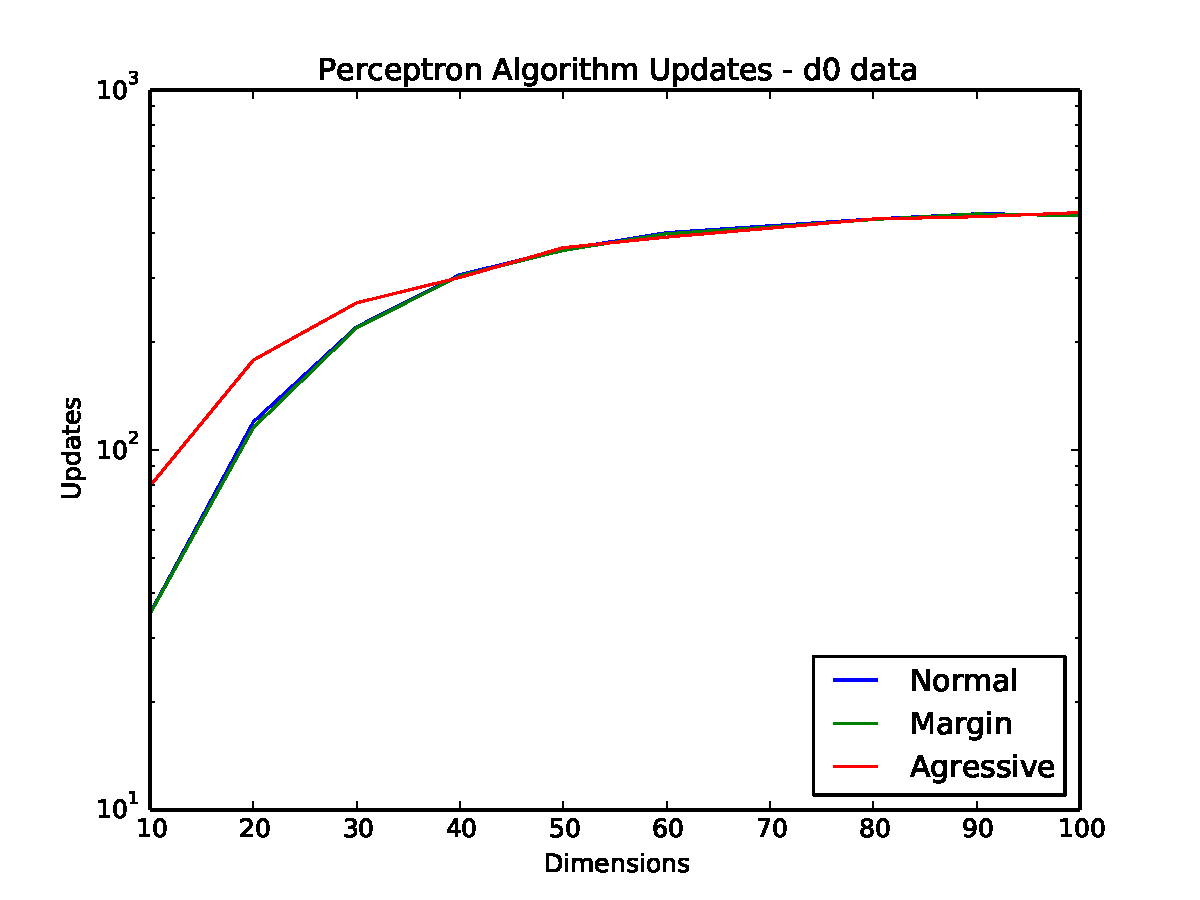
\includegraphics[width=\linewidth]{d0_updates.pdf}
  \captionof{figure}{Updates for {\tt data0}}
  \label{fig:updates_d0}
\end{minipage}%
\begin{minipage}{.5\textwidth}
  \centering
  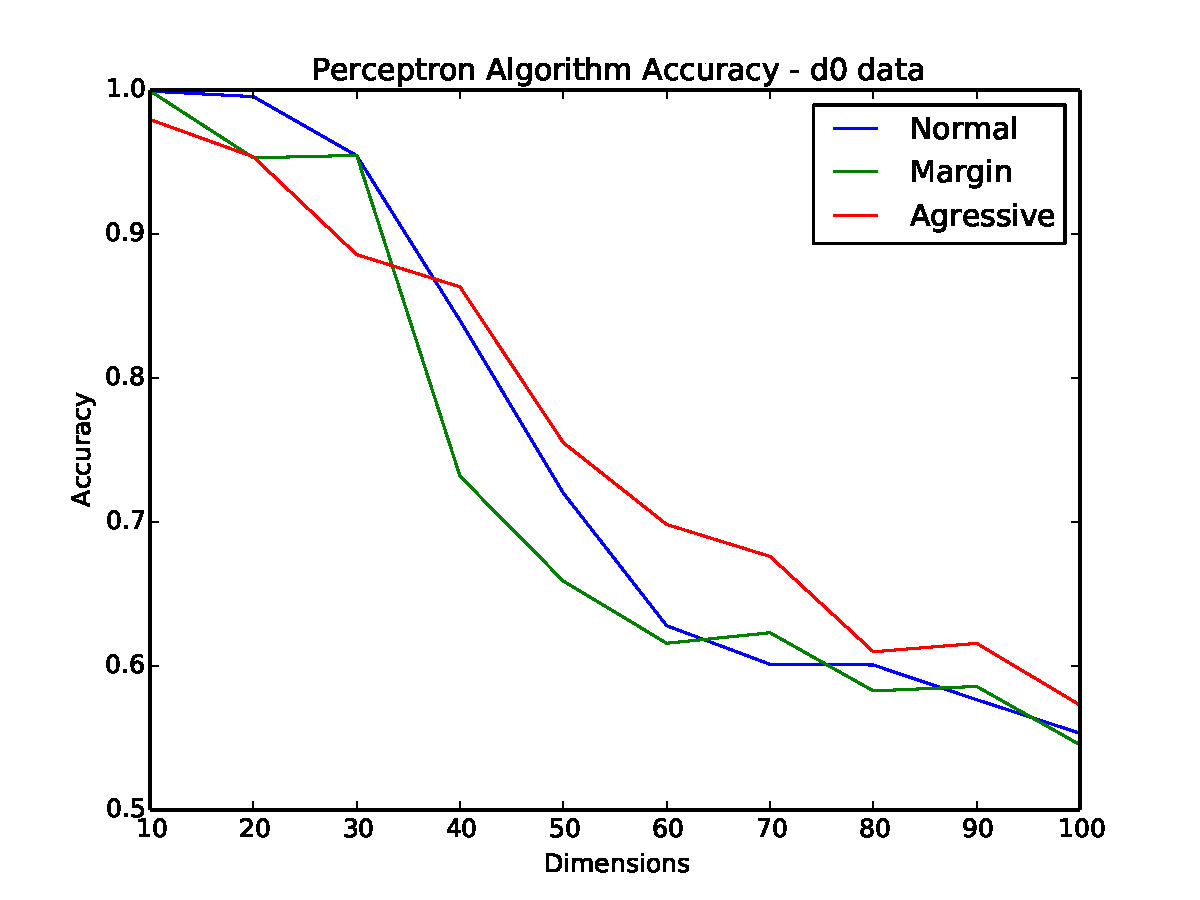
\includegraphics[width=\linewidth]{d0_accuracy.pdf}
  \captionof{figure}{Accuracy for {\tt data0}}
  \label{fig:accuracy_d0}
\end{minipage}
\end{figure}

Figure \ref{fig:updates_d0} shows the number of updates per algorithm for each of
the different Perceptron algorithms vs the dimensionality. This is only for the
dataset in \verb~data0~. As can be seen in the figures, the Margin Perceptron and
Normal Perceptron performed roughly the same, while the Agressive Perceptron required
more updates than either of the others, after which it performed roughly the same.

Seeing how this effects the accuracy in Figure \ref{fig:accuracy_d0}, up through 40
dimensions the Agressive Perceptron performs worse than the first two algorithms.
However, even though this is the case, the overall accuracy of the Agressive algorithm
drops off roughly linearly with the number of dimensions, while the other algorithms
drop off much quicker in accuracy for the dimensionality greater than 40.

\begin{figure}[H]
\centering
\begin{minipage}{.5\textwidth}
  \centering
  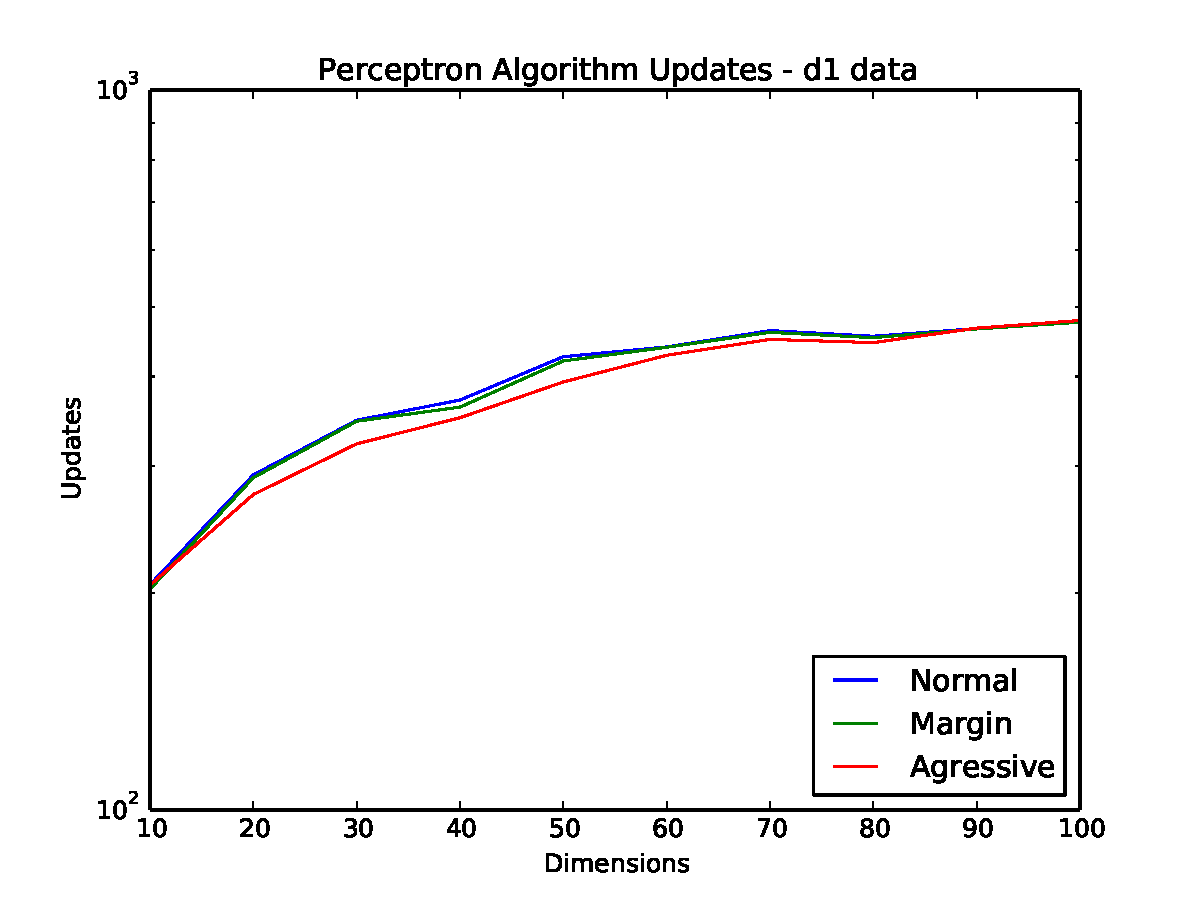
\includegraphics[width=\linewidth]{d1_updates.pdf}
  \captionof{figure}{Updates for {\tt data1}}
  \label{fig:updates_d1}
\end{minipage}%
\begin{minipage}{.5\textwidth}
  \centering
  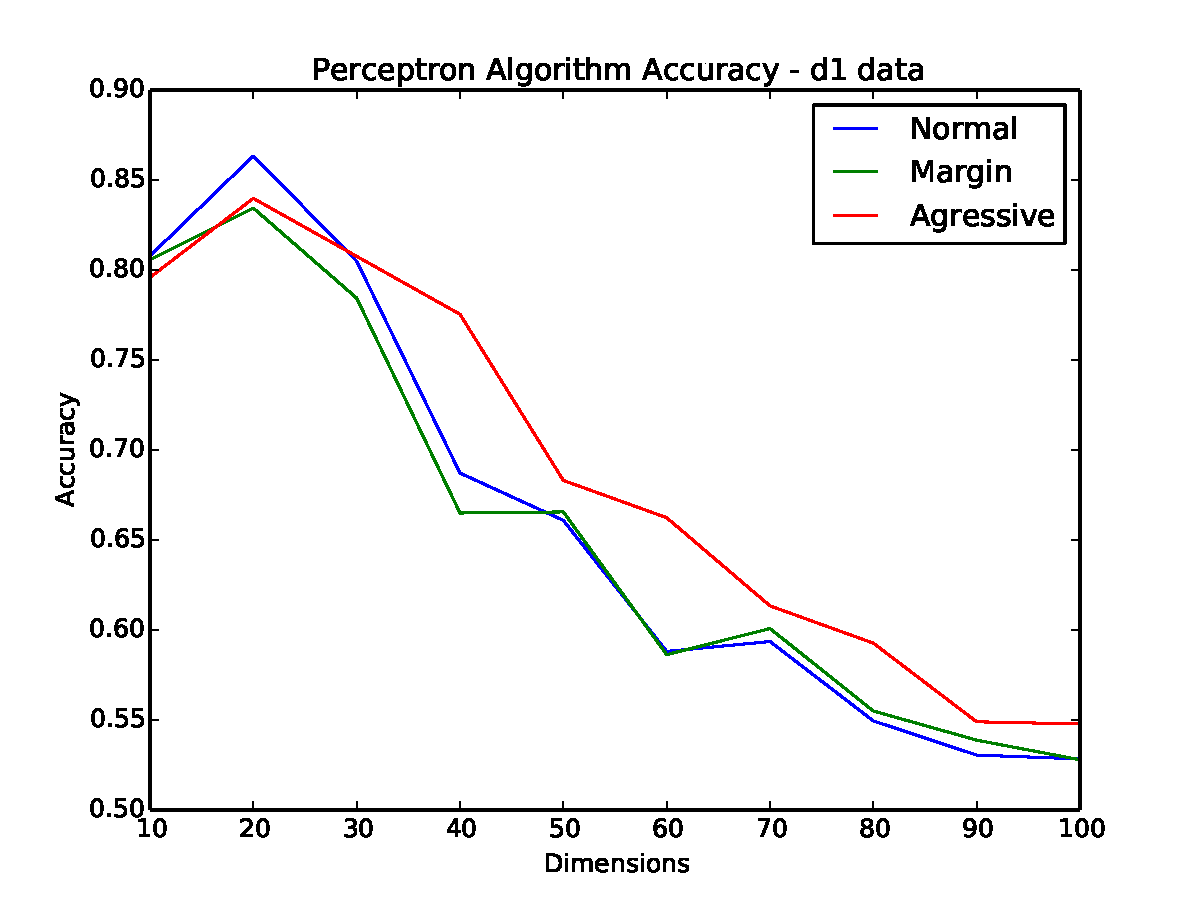
\includegraphics[width=\linewidth]{d1_accuracy.pdf}
  \captionof{figure}{Accuracy for {\tt data1}}
  \label{fig:accuracy_d1}
\end{minipage}
\end{figure}

Figure \ref{fig:updates_d1} shows the number of updates for each of the different
Perceptron algorithms vs dimensionality for \verb~data1~. The difference between
this set of data and the first set is that for the number of updates the Agressive
Perceptron algorithm seems to do better when looking at the number of updates.
The Margin Perceptron and Normal Perceptron perform relatively the same.

The results of this shows up in \ref{fig:accuracy_d1}. When compared to the accuracy
that is in Figure \ref{fig:accuracy_d0} from \verb~data0~, all of the algorithms
perform much less accurate than their counterparts in Figure \ref{fig:accuracy_d0}.
However, the drop in the amount of accuracy is much more for both the Margin Perceptron
and the Normal Perceptron Algorithms. In other words, the Agressive Perceptron algorithm
performed much better than the other two in this data set, which was not the case for
\verb~data0~.

Overall, out of the 3 different algorithms, the Agressive Perceptron algorithm
performs better for higher dimensional data when compared to either of the other two.
This is most likely because when updating the weight vector with $\eta$, you're dividing by the norm of $x$ which allows for it to be less susceptible to noise. On top of this, the Agressive
Perceptron also did better than both in \verb~data1~ than \verb~data0~ and did
not loose as much in accuracy. Again, this is most likely because of there being more noise in the second set of data and the agressive persceptron is less sensitive to this.
The Agressive Perceptron Algorithm seems to drop of linearly with respect to the dimensions
while the other two are more sensitive to the number of dimensions.


  \paragraph{Explanation of the update} We call this the aggressive
  update because the learning rate is derived from the following
  optimization problem:

  When we see that $y(\bw^T \bx) \leq \mu$, we try to find new values
  of $\bw$ such that $y(\bw^T \bx) = \mu$ using
  %
  \begin{eqnarray*}
    \min_{\bw_{new}} &     \frac{1}{2} {||\textbf{$\bw_{new}$} - \textbf{$\bw_{old}$}||}^2\\
    \mbox{such that} & y(\bw^T x) = \mu.
  \end{eqnarray*}
  %
  That is, the goal is to find the smallest change in the weights so
  that the current example is on the right side of the weight vector.

  By substituting (a) from above into this optimization problem, we
  will get a single variable optimization problem whose solution gives
  us the $\eta$ defined above. You can think of this algorithm as
  trying to tune the weight vector so that the current example is
  correctly classified right after the update.
\end{enumerate}


\subsection*{Submission Guidelines}

\begin{enumerate}
\item The report should detail your experiments. For each step,
  explain in no more than a paragraph or so how your implementation
  works.

\item {\em Your code should run on the CADE machines}. You should
  include a shell script, {\tt run.sh}, that will execute your code
  in the CADE environment. Your code should produce similar output
  to what you include in your report.

  You are responsible for ensuring that the grader can execute the
  code using only the included script. If you are using an
  esoteric programming language, you should make sure that its
  runtime is available on CADE.


\item Please do not hand in binary files! We will {\em not} grade
  binary submissions.

\end{enumerate}

%%% Local Variables:
%%% mode: latex
%%% TeX-master: "hw2"
%%% End:


\end{document}
%%% Local Variables:
%%% mode: latex
%%% TeX-master: t
%%% End:
